\def\assignmenttitle{Consumer evaluations of carrots}
\def\assignmentdate{24-10-2011}
\def\coursetitle{02418 Statistical modelling}
\def\Consumer{\myverb{Consumer}}
\def\product{\myverb{product}}
\def\Sweetness{\myverb{Sweetness}}
\def\age{\myverb{age}}
\def\gender{\myverb{gender}}
\def\cultivar{\myverb{cultivar}}
\def\region{\myverb{region}}
\def\plotfolder{../plots}

\documentclass[11pt]{article}
\linespread{1}

\renewcommand{\thefootnote}{\fnsymbol{footnote}}

\usepackage{geometry} % see geometry.pdf on how to lay out the page. There's lots.
\usepackage[utf8]{inputenc}
\usepackage[T1]{fontenc}
\usepackage{array}
\usepackage{amsmath,amssymb,latexsym,epic,eepic,epsfig,graphics,psfrag}
\usepackage{amsfonts}
\usepackage{graphicx,float}
\usepackage{color}
\definecolor{mygray}{RGB}{244,244,244}
\definecolor{gray}{gray}{0.5}
\definecolor{myredish}{RGB}{193,33,97}
\definecolor{grayblue}{RGB}{91,112,142}
\definecolor{myorange}{RGB}{255,134,0}
\definecolor{green}{rgb}{0,0.4,0}

\usepackage[english]{babel}

\usepackage[bottom]{footmisc}

\usepackage{fancyhdr}
\pagestyle{fancy}
\lhead{\small\textit{Assignment \assignmentnumber -- 02417 Time Series Analysis -- Anders Hørsted (s082382)}}
\rhead{\thepage}
\chead{}
\lfoot{}\cfoot{}\rfoot{}

\usepackage{subfigure}
\usepackage{pstricks}
\usepackage{pst-node}
\usepackage{wrapfig}
\usepackage{caption}
\usepackage{multirow}
%\usepackage{fouriernc}
%\usepackage[charter]{mathdesign}
\usepackage{lmodern}
\usepackage[normalem]{ulem}
\geometry{a4paper} % or letter or a5paper or ... etc
% \geometry{landscape} % rotated page geometry

\usepackage{url}


\makeatletter
\renewcommand*\env@matrix[1][*\c@MaxMatrixCols c]{%
  \hskip -\arraycolsep
  \let\@ifnextchar\new@ifnextchar
  \array{#1}}
\makeatother

\newcommand\myimp{\quad\Leftrightarrow\quad}
\newcommand\half{\frac{1}{2}}
\newcommand\myvec[1]{\mathbf{#1}}
\newcommand\mymod[1]{\ (\text{mod }#1)}
\newcommand\myreal{\mathbb{R}}
\newcommand\mynatural{\mathbb{N}}
\newcommand\myinteger{\mathbb{Z}}
\newcommand\mycomplex{\mathbb{C}}
\newcommand\myint{\text{int}}
\newcommand\norm[1]{||\,#1\,||}
\newcommand\bignorm[1]{\big|\big|\,#1\,\big|\big|}
\newcommand\seq[1]{\big\{#1\big\}}
\newcommand\smallseq[1]{\{#1\}}
\newcommand\smallseqtoinf[1]{\smallseq{#1}_{k=1}^\infty}
\newcommand\lonew{\ell^1_w}
\newcommand\lone{\ell^1}
\newcommand\ltwo{\ell^2(\mynatural)}
\newcommand\ip[2]{\langle#1,#2\rangle}
\newcommand\hilbert[1]{\mathcal{#1}}
\newcommand\uinf{u_{\infty}}
\newcommand\erf{\text{erf\,}}
\newcommand\infint{\int_{\infty}^{\infty}}
\newcommand\fpi{FPI}
\newcommand\E[1]{\text{E}[#1]}
\newcommand\Var[1]{\text{Var}[#1]}
\newcommand\Cov[1]{\text{Cov}[#1]}
\newcommand\myverb[1]{{\footnotesize\texttt{#1}}}
\newcommand\Yhat{\widehat{Y}}
\newcommand\given{\,|\,}

\usepackage[scaled]{beramono}
\usepackage{listings}
\lstset {                 % A rudimentary config that shows off some features.
    language=R,
    basicstyle=\scriptsize\ttfamily, % Without beramono, we'd get cmtt, the teletype font.
    commentstyle=\textit, % cmtt doesn't do italics. It might do slanted text though.
    keywordstyle=,
    identifierstyle=,
    framextopmargin=4pt,
    framexbottommargin=4pt,
    framexleftmargin=4pt,
    framexrightmargin=4pt,
    xleftmargin=4pt,
    xrightmargin=4pt,
    backgroundcolor=\color{mygray},
    frame=single,
    showstringspaces=false,
    captionpos=b,
    tabsize=4            % Or whatever you use in your editor, I suppose.
}

\renewcommand{\lstlistlistingname}{Code Listings}
\renewcommand{\lstlistingname}{Code Listing}

\usepackage{tabulary}
\newcolumntype{y}{>{\centering\arraybackslash}R}

\title{\assignmenttitle}
\date{\assignmentdate}
\author{Assignment \assignmentnumber\ -- 02417 Time Series Analysis -- Anders Hørsted (s082382)}
%\author{}
\date{} % delete this line to display the current date




\begin{document}

\maketitle

In this case a data set with consumer evaluations of carrots are given. Each consumer (103 in total) have evaluated carrots of 6 different cultivars from 2 different regions. Each combination of cultivar and region is called a product. Based on the data set we will examine the relationship between various traits of the consumers (eg. age, gender etc.) and how they score the carrots. Specifically we will focus on the sweetness score.

\section*{Question 1}
In the first question we focus on the two factors consumer and product and examine whether there are any differences in sweetness scores between different consumers and/or products. To get an overview of the data a histogram of the sweetness scores is plotted. Also boxplots of the sweetness scores grouped by product and consumer are plotted. All three plot are seen in figure~\ref{fig:hist-and-boxplot}. It is seen that there are large differences between the median scores of the different consumers. This is expected since the scoring of the sweetness is a subjective measure and the perception of different consumers is bound to differ. The differences between the specific consumers isn't very interesting but as a confounding variable it is important that we control for the differences. From the plots there also seems to be differences between the median sweetness of the various products. This is of cause interesting and we will therefore perform an ANOVA to determine whether the differences are significant or not.

\begin{figure}
    \centering
    \mbox{  \subfigure{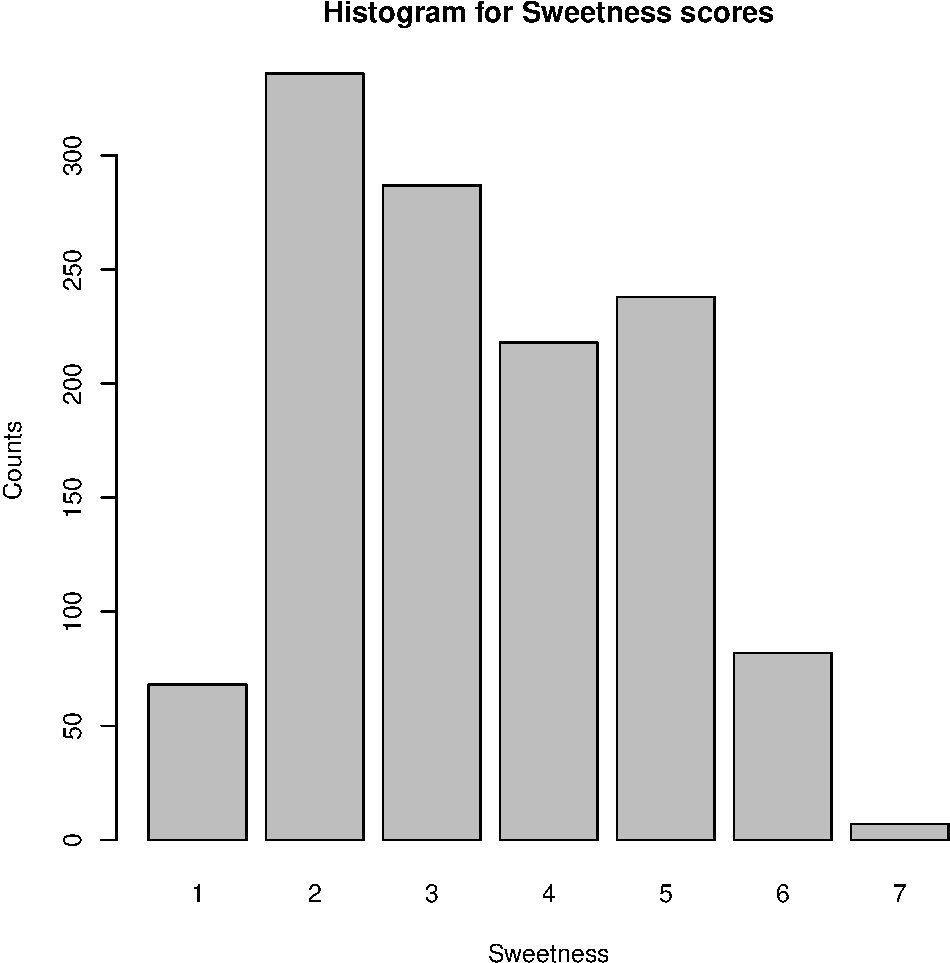
\includegraphics[width=70mm]{\plotfolder/sweetness-histogram.pdf}} \quad 
            \subfigure{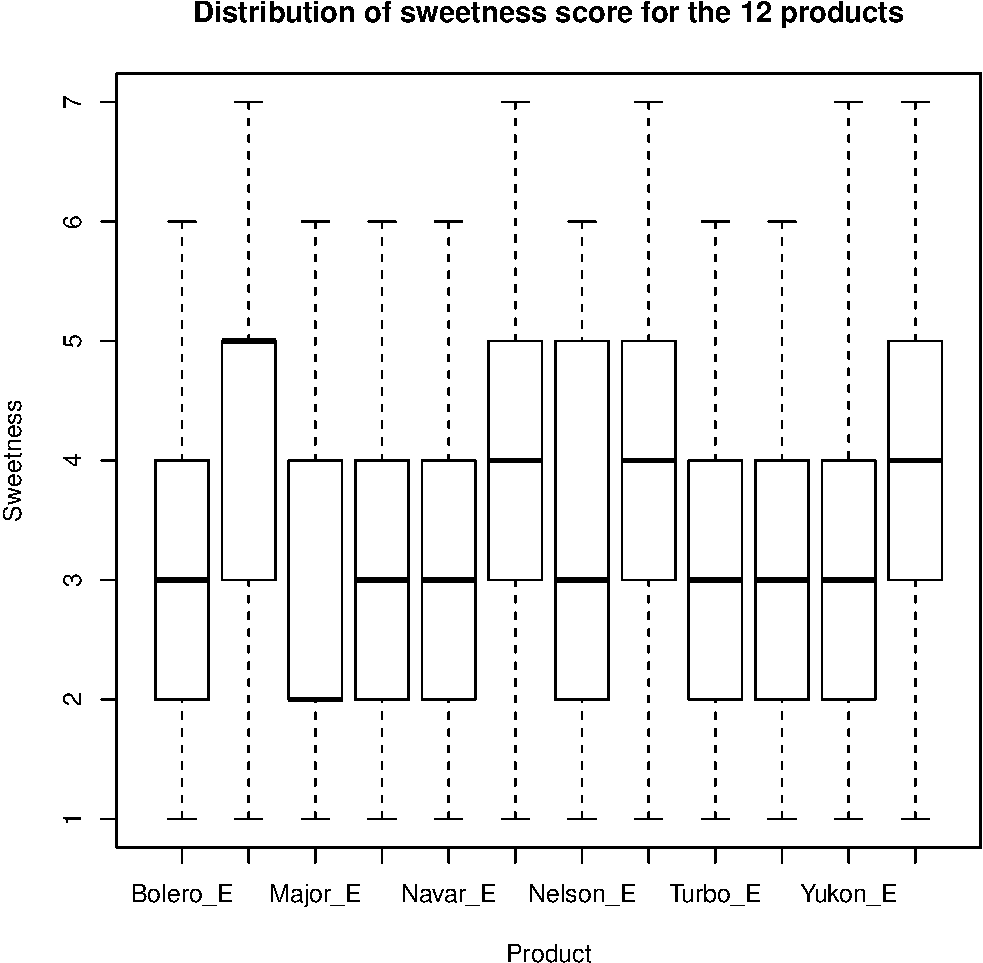
\includegraphics[width=70mm]{\plotfolder/product-boxplot.pdf}}}
    \mbox{  \subfigure{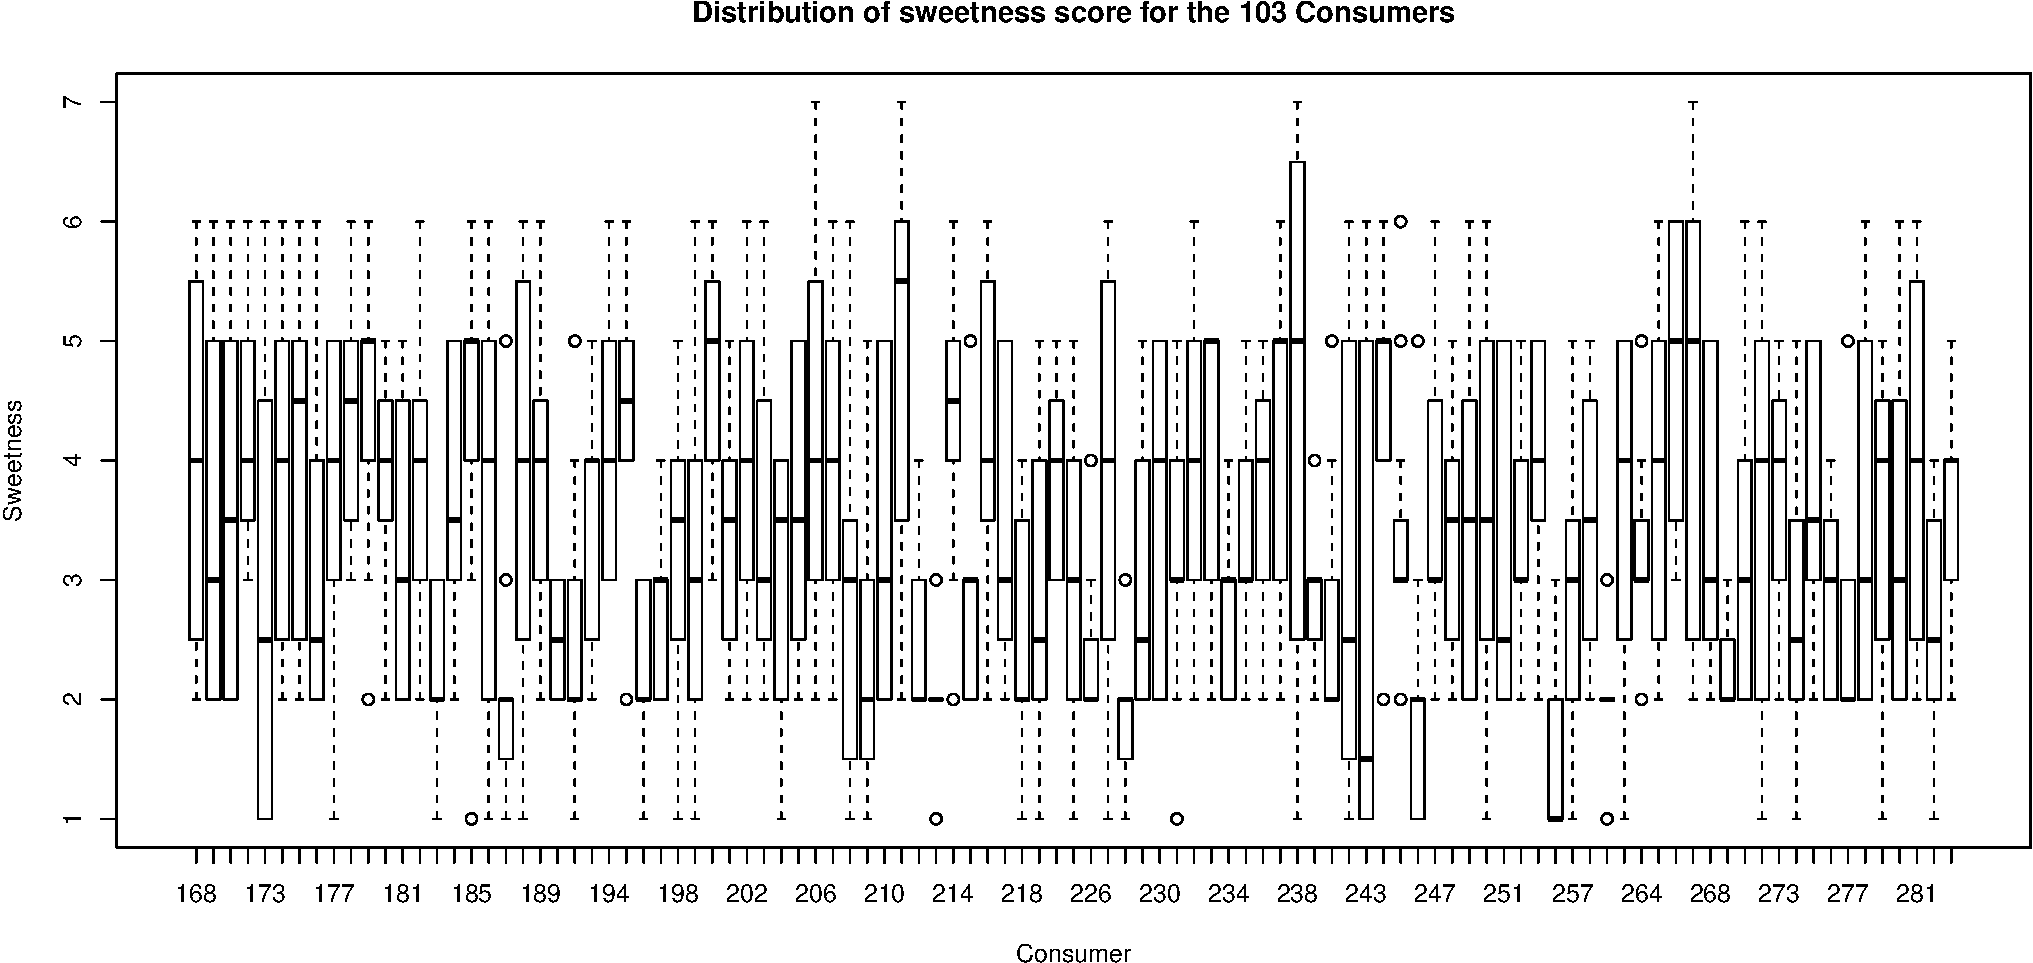
\includegraphics[width=150mm]{\plotfolder/consumer-boxplot.pdf}}}
    \caption{Histogram for sweetness score and boxplots for the product and consumer factor}
    \label{fig:hist-and-boxplot}
\end{figure}

\subsection*{Performing an ANOVA}
To perform the ANOVA a model is defined as \myverb{Sweetness\texttildelow Consumer+product}. The \myverb{anova} function is called on the model and gives the output in table~\ref{tbl:q1-anova1}. It is seen that the means of some consumers are not equal as well as some of the means of products are nor equal.
\begin{table}
    \centering
    % latex table generated in R 2.10.1 by xtable 1.5-6 package
% Tue Oct 25 09:57:57 2011
\begin{tabular}{lrrrrr}
  \hline
 & Df & Sum Sq & Mean Sq & F value & Pr($>$F) \\ 
  \hline
Consumer & 102 & 632.29 & 6.20 & 4.60 & 0.0000 \\ 
  product & 11 & 284.57 & 25.87 & 19.20 & 0.0000 \\ 
  Residuals & 1122 & 1512.10 & 1.35 &  &  \\ 
   \hline
\end{tabular}

    \caption{ANOVA table for the two way ANOVA on the Consumer and product factors}\label{tbl:q1-anova1}
\end{table}

Before starting on the post-hoc analysis the model assumptions are checked by plotting a QQ-plot and a residual plot (see figure~\ref{fig:qq-and-residuals}). The QQ-plot seems to confirm that the errors are normal distributed. The residual plot is a bit difficult to interpret due to the fact that Sweetness is actually a discrete variable. The residuals are independent of the fitted values (see \cite[p.85]{bingham10}) so no pattern should be recognizable in a fitted values vs. residuals plot. There is obivous some pattern in the residual plot in figure~\ref{fig:qq-and-residuals} and you could argue that variance is smaller for fitted values near 1 and 7, and larger for fitted values near 3.5. Using the R function \myverb{boxcox} a transformation by $(y^{0.5} - 1)/0.5$ was attempted on the Sweetness response, but the resulting QQ-plot showed greater deviation from normality and no improvement in the residuals plot was found (see \appref{transformations-model1}). The result is that the original model is accepted. The next step is a post-hoc analysis.

\begin{figure}
    \centering
    \mbox{  \subfigure{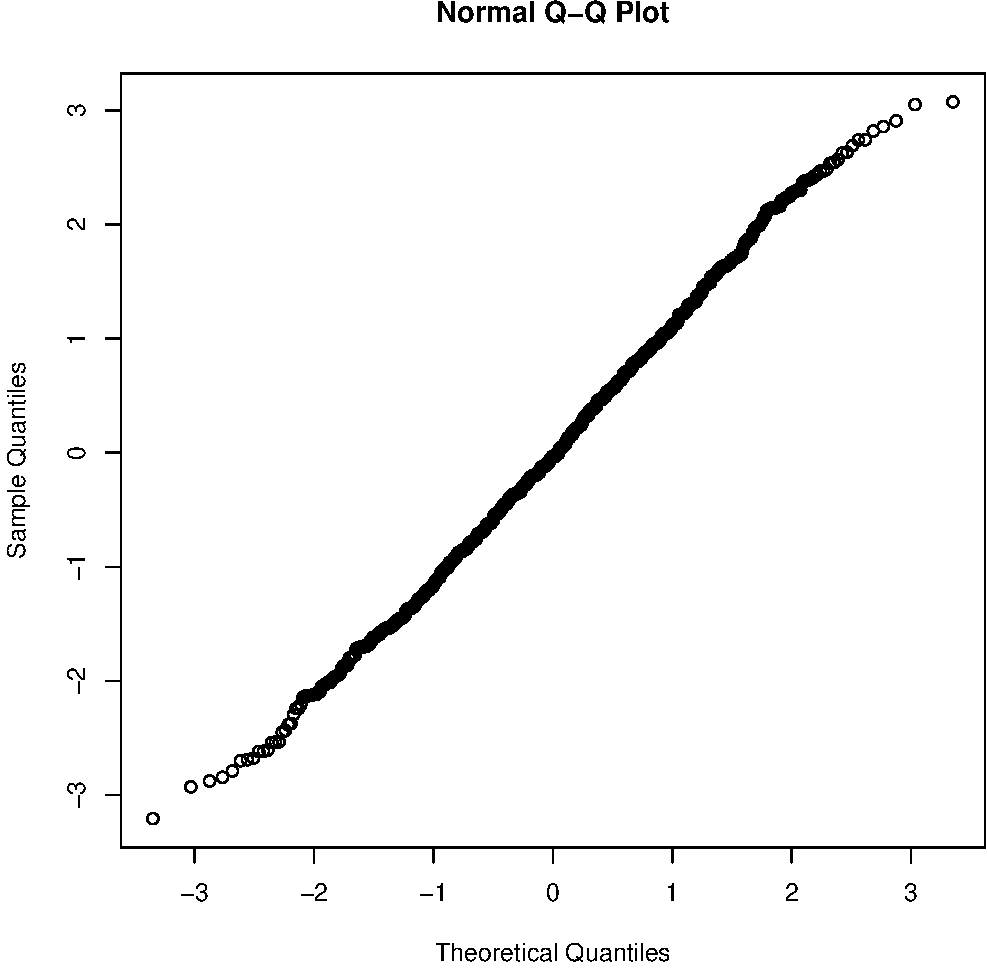
\includegraphics[width=70mm]{\plotfolder/qqplot-model1.pdf}} \quad 
            \subfigure{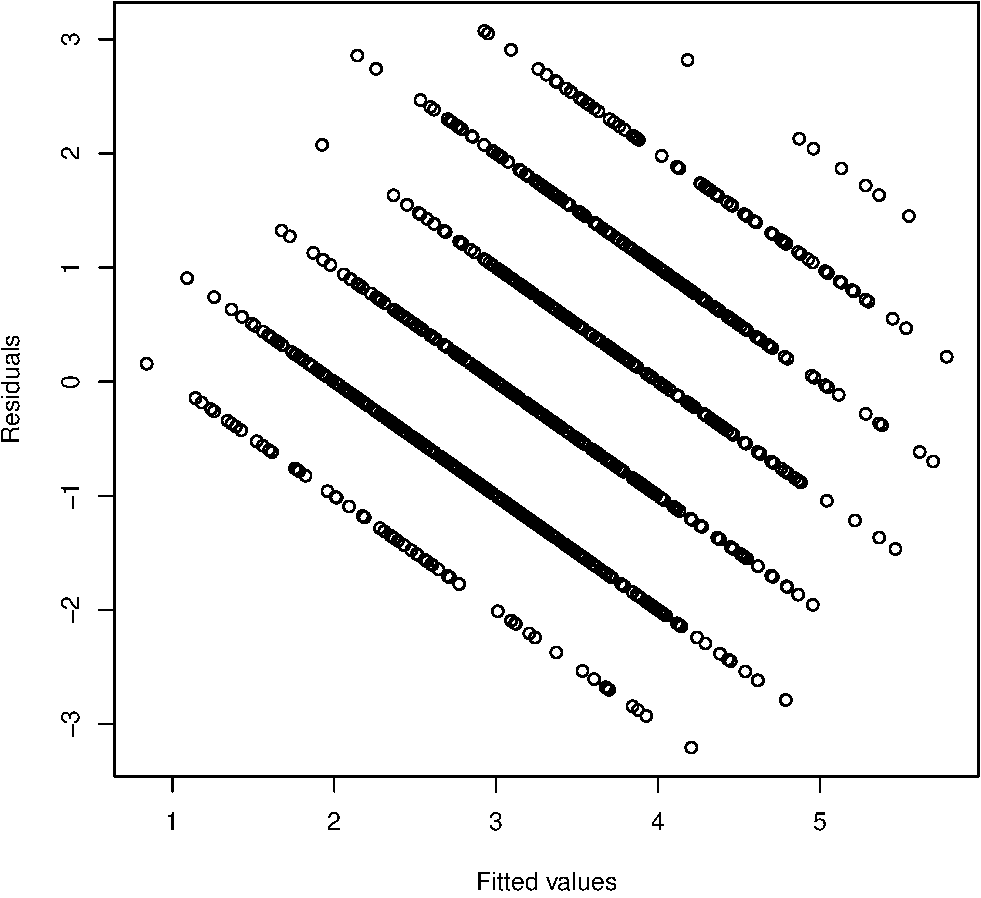
\includegraphics[width=70mm]{\plotfolder/residuals-model1.pdf}}}
    \caption{Diagnostic plots for the two way ANOVA on the Consumer and product factors}
    \label{fig:qq-and-residuals}
\end{figure}

\subsubsection*{Post-hoc analysis}
Since we are not interested in determining which consumers have significantly different means we only look at the differences between all pairs of products. With 12 products we need to perform $\frac{12\cdot 11}{2}=66$ t-tests, but with the standard 5\% chance of an type I we would expect 3-4 significant differences by chance alone. To correct for the multiple comparison a Tukey Range Test is performed on all 66 pairs of products and it is found that a total of 31 pairs have significantly different means. The results are shown in \appref{q1-tukey}. From the results it seems as if the Bolero cultivar is sweeter than most other cultivars except for maybe Yukon. Also the region Lammefjord seem to consistently score higher on sweetness than the other region Ejstrupholm. It isn't 100\% clear though so a natural next step is to make an ANOVA with region and cultivar as separate factors.


\section*{Question 2}
We now look at the region and cultivar as separate factors. To get an overview of these two factors and to look for possible interaction between the two factors an interaction plot for the factors are now plotted in figure~\ref{fig:interaction-cultivar-region}. The interaction plot supports that the region Lammefjord makes sweeter carrots than Ejstrupholm. There also seems to be interactions between the region and cultivar since the lines in the interaction plot isn't parallel. Eg. the increase in sweetness between Ejstrupholm and Lammefjord is larger for the bolero and yukon cultivar than for the other cultivars. It will therefore make sense to try and fit a model with interactions. \par

\begin{figure}[ht]
    \centering
    \mbox{  \subfigure{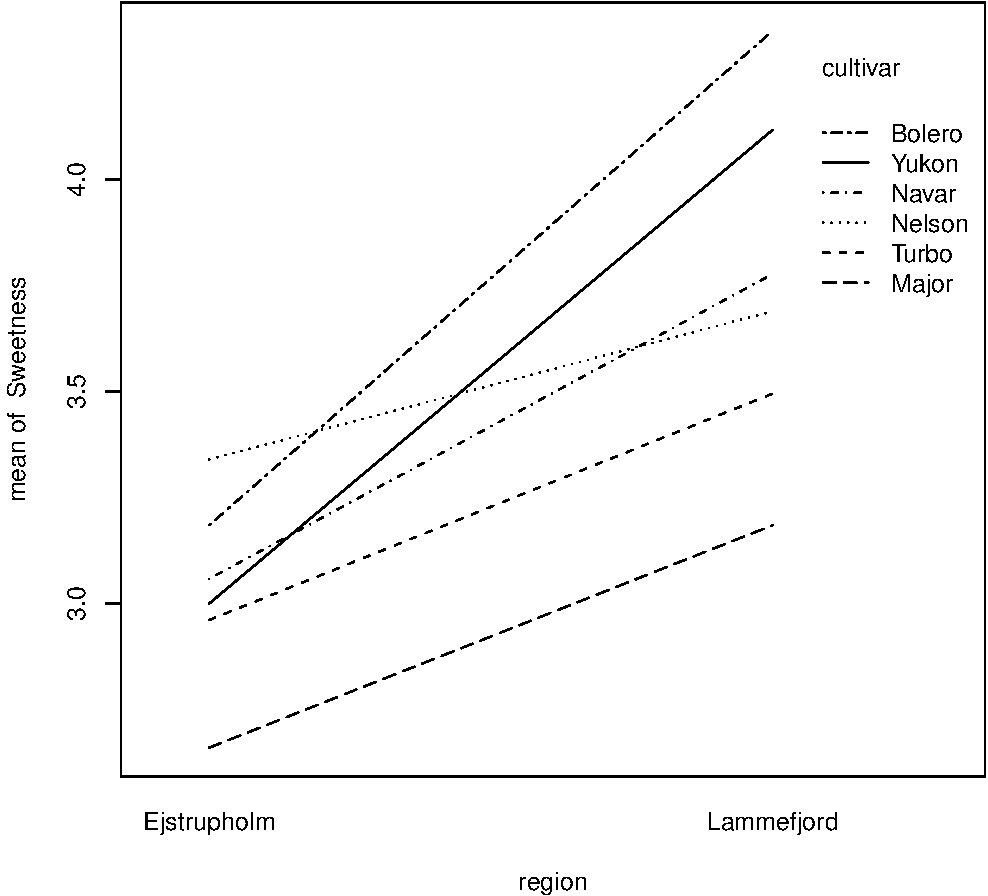
\includegraphics[width=70mm]{\plotfolder/interaction-region-cultivar.pdf}}}
    \caption{Interactions between cultivar and region}
    \label{fig:interaction-cultivar-region}
\end{figure}

By entering the model \myverb{Sweetness\texttildelow Consumer+cultivar*region} and running the \myverb{anova} function we get the output shown in table~\ref{tbl:anova-model2}. From the results there seems to be significant differences in the means for both the cultivar and region factor as well as the interactions. Since there are only two regions it can be concluded by looking at the coefficients of the model, that the region Lammefjord grows significantly sweeter carrots than Ejstrupholm. To find which cultivar that differs a Tukey's range test is performed on the cultivar factor. From the results (see \appref{q2-tukey}) we find that the only significant results are that Bolero is sweeter than Major and that Nelson is sweeter than Major. This result isn't exactly what was expected based on the results in question 1. In question 1 it was anticipated that Bolero would be sweeter than all other cultivars except for Yukon. It turns out only the difference between Bolero and Major is significant. \par
The main conclusion of these two first ANOVAs must be that the Lammefjord region grows sweeter carrots than Ejstrupholm.

\begin{table}
    \centering
    % latex table generated in R 2.10.1 by xtable 1.5-6 package
% Tue Oct 25 12:13:47 2011
\begin{tabular}{lrrrrr}
  \hline
 & Df & Sum Sq & Mean Sq & F value & Pr($>$F) \\ 
  \hline
Consumer & 102 & 632.29 & 6.20 & 4.60 & 0.0000 \\ 
  cultivar & 5 & 88.75 & 17.75 & 13.17 & 0.0000 \\ 
  region & 1 & 166.76 & 166.76 & 123.74 & 0.0000 \\ 
  cultivar:region & 5 & 29.06 & 5.81 & 4.31 & 0.0007 \\ 
  Residuals & 1122 & 1512.10 & 1.35 &  &  \\ 
   \hline
\end{tabular}

    \caption{ANOVA table for the model in question 2}\label{tbl:anova-model2}
\end{table}

\section{Question 3}
We now look at the two consumer factors age and gender and try to see if there are any differences within these two factors for how they score the sweetness of carrots.

\textit{Due to bad time management this is unfortunately how far I get before hand-in.}

\pagebreak

\renewcommand\thesection{\Alph{section}}
\section{Appendices}
All R source code is included in the appendices. All the source code including the Latex code used for the report can also be found at \url{https://github.com/alphabits/dtu-fall-2011/tree/master/02418/carrots}.
\subsection{Diagnostic plots for model with transformed response}\label{app:transformations-model1}
\begin{figure}[ht]
    \centering
    \mbox{  \subfigure{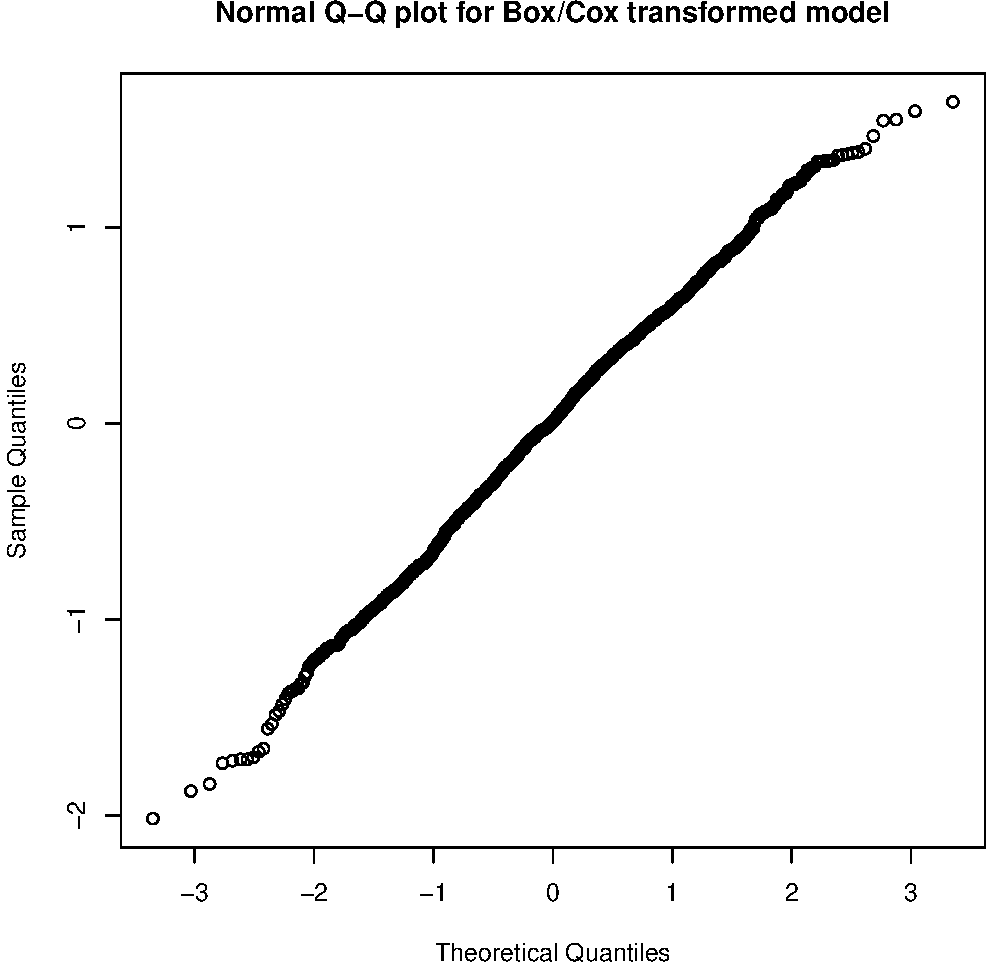
\includegraphics[width=70mm]{\plotfolder/qqplot-model-boxcox.pdf}} \quad 
            \subfigure{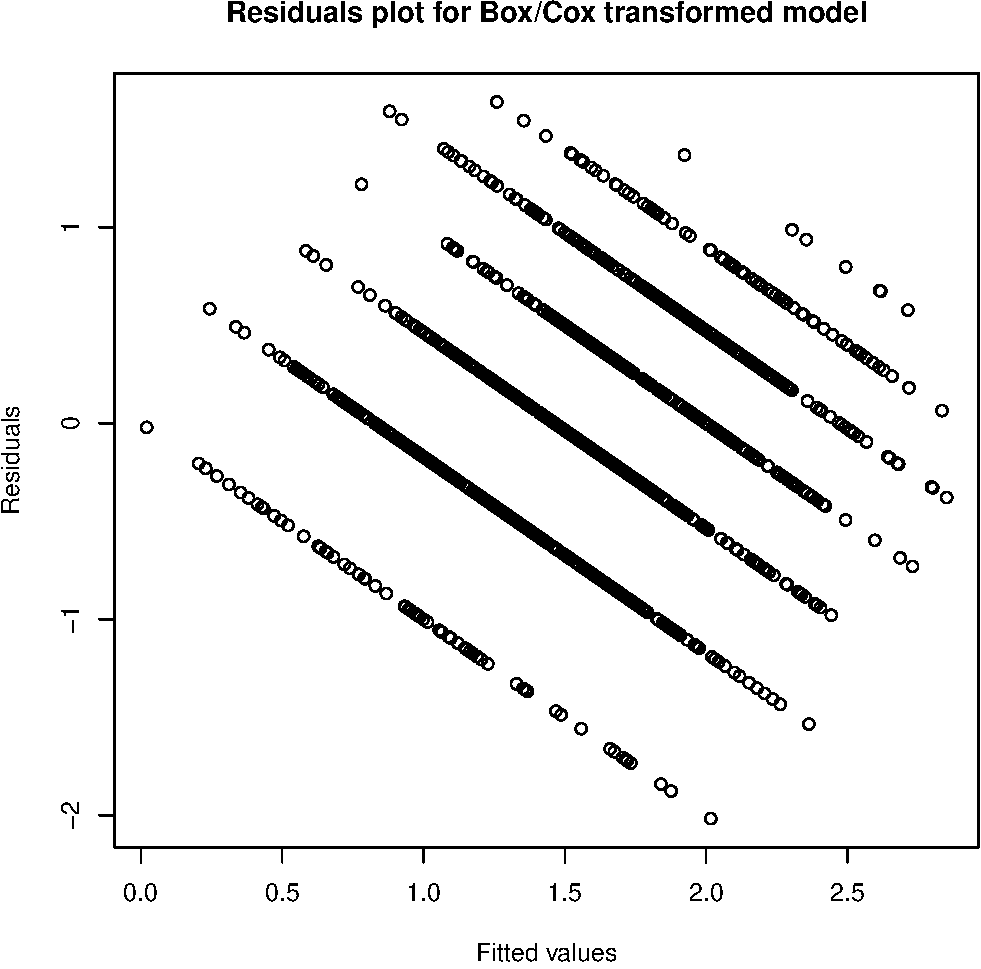
\includegraphics[width=70mm]{\plotfolder/residuals-model-boxcox.pdf}}}
%    \mbox{  \subfigure{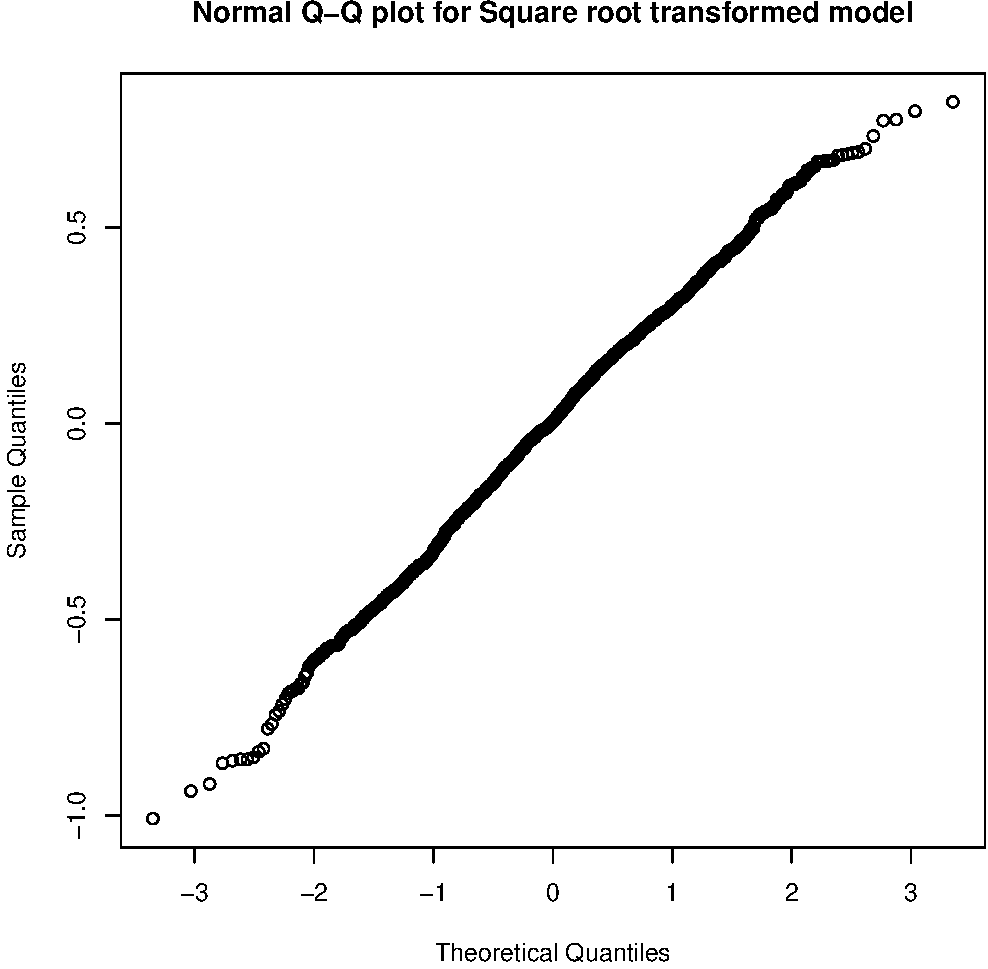
\includegraphics[width=70mm]{\plotfolder/qqplot-model-sqrt.pdf}} \quad 
%            \subfigure{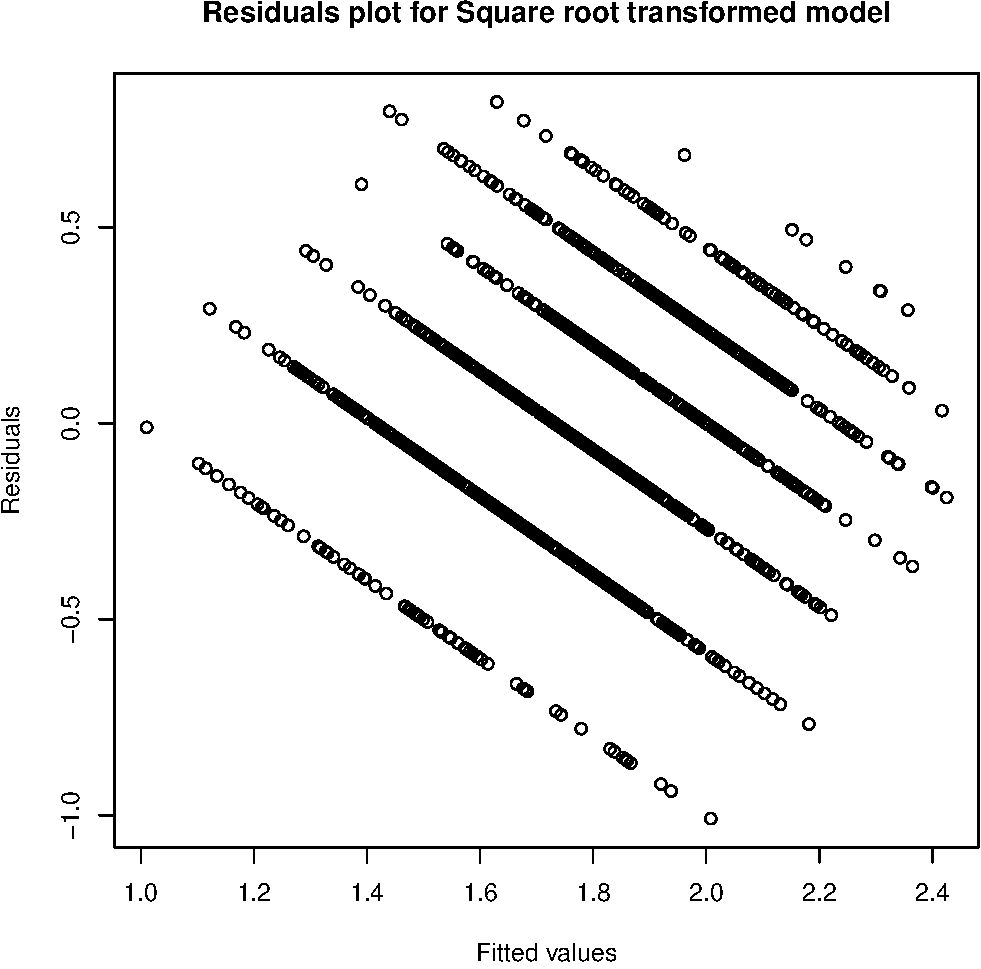
\includegraphics[width=70mm]{\plotfolder/residuals-model-sqrt.pdf}}}
%    \mbox{  \subfigure{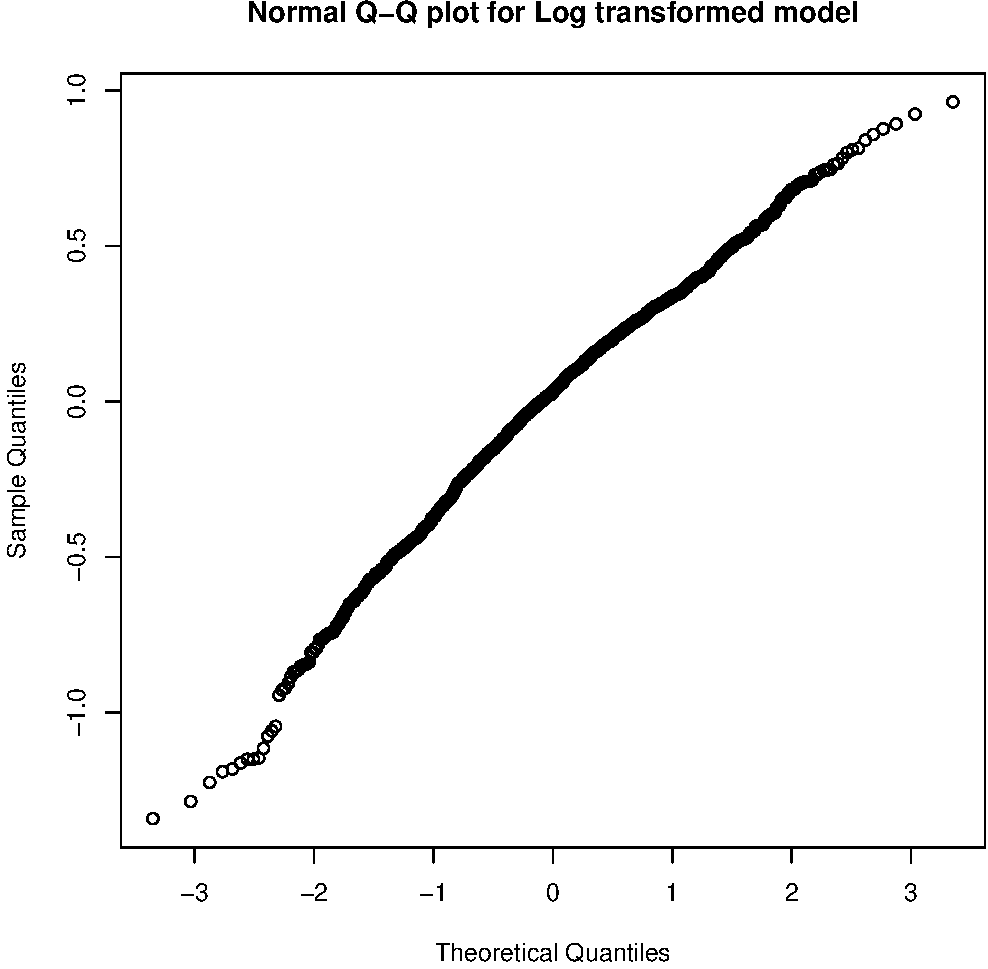
\includegraphics[width=70mm]{\plotfolder/qqplot-model-log.pdf}} \quad 
%            \subfigure{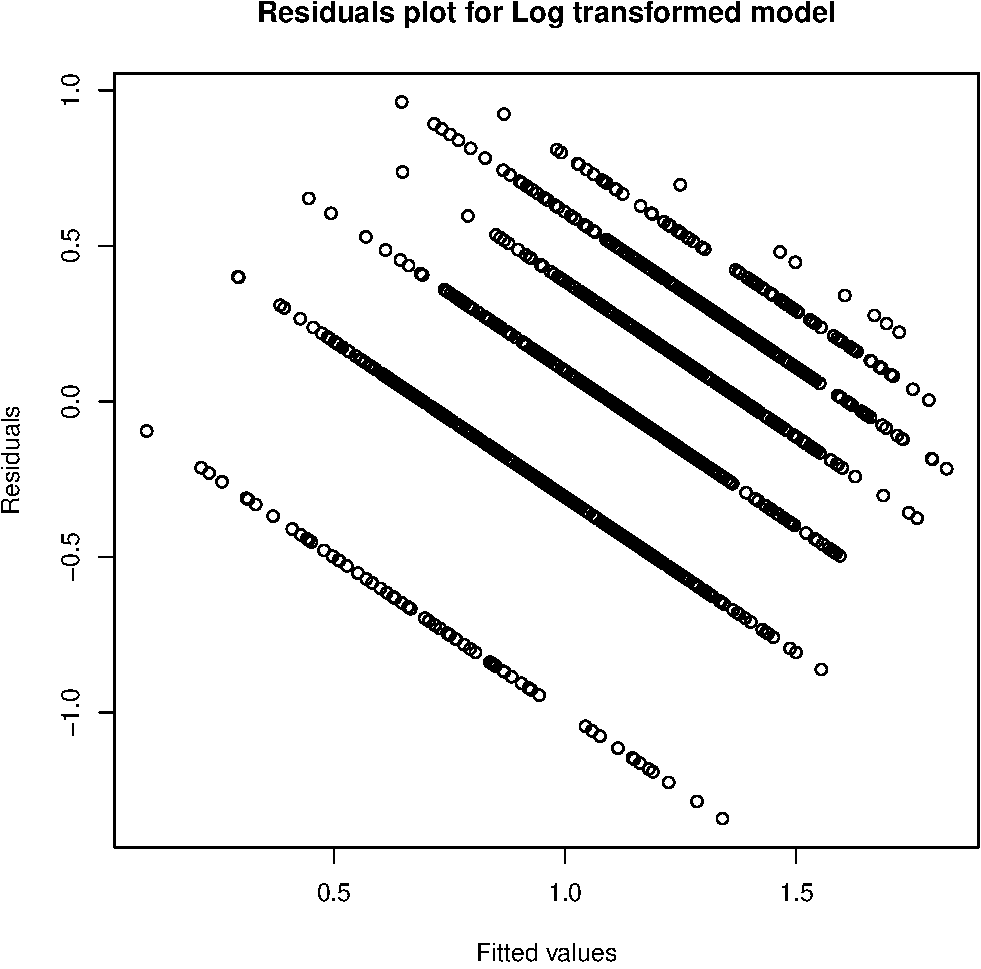
\includegraphics[width=70mm]{\plotfolder/residuals-model-log.pdf}}}
    \caption{QQ plot and residuals for the Box/Cox transformed model}
    \label{fig:qq-and-residuals-log-sqrt}
\end{figure}
\subsection{functions.R}
\lstinputlisting{../src/functions.R}
\subsection{loaddata.R}
\lstinputlisting{../src/loaddata.R}
\subsection{question1.R}
\lstinputlisting{../src/question1.R}
\subsection{question2.R}
\lstinputlisting{../src/question2.R}
\subsection{Results of Tukey's range test for question 1}\label{app:q1-tukey}
Only comparisons with a p-value less than 10\% are included.
\lstinputlisting{../tables/q1-post-hoc-trimmed.tex}
\subsection{Results for Tukey's range test for question 2}\label{app:q2-tukey}
\lstinputlisting{../tables/q2-post-hoc-trimmed.tex}

\pagebreak
\begin{thebibliography}{9}

\bibitem{hm}
  Henrik Madsen,
  \emph{Time Series Analysis}.
  Chapman \& Hall/CRC,
  1st Edition,
  2008.

%\bibitem{taleb}
%  Nassim Nicholas Taleb,
%  \emph{The Black Swan}.
%  Random House Trade Paperbacks
%  2nd Edition,
%  2010.

\end{thebibliography}


\end{document}
